\section{Compression as Anchored Continuation}
\label{sec:method}

\begin{figure*}[t]
\centering
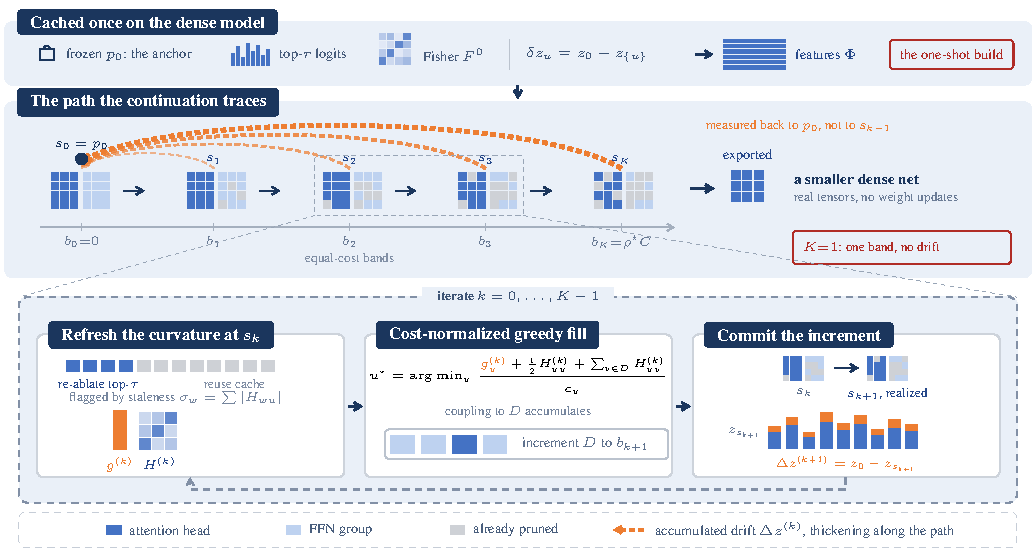
\includegraphics[width=0.9\textwidth]{figs/fig_overview.pdf}
\caption{\textbf{Overview of \method.} One calibration pass caches the frozen teacher and one ablation feature per unit (\emph{top}). The continuation traces the removal-cost path from $s_0{=}\mathbf{0}$ to $s_K$, always measuring damage against the fixed anchor $p_0$ (\emph{middle}). At each step (\emph{bottom}) it refreshes only the stalest units, forms $\Hmat^{(k)}$ and the drift term $g^{(k)}$, and fills the band by a cost-normalized greedy. At $K{=}1$ the drift vanishes and the method reduces to one-shot second-order pruning.}
\label{fig:method}
\end{figure*}

\subsection{The Anchored Continuation}
One-shot pruning builds a single quadratic at the dense model and extrapolates it across the whole
budget. \method instead follows the cost-indexed path in Fig.~\ref{fig:method} (\emph{middle}), with each
transition implemented by the refresh--select--commit loop shown at the \emph{bottom}. We call this
discrete budget-indexed rebuilding an \emph{anchored continuation}:
the dense teacher and its Fisher metric stay fixed while selection walks a \emph{path} through changing
operating points. Throughout, $s\in\{0,1\}^M$ is the
\emph{removal} indicator ($s_u{=}1$ means unit $u$ is pruned) and $\delta$ the increment removed at the
current step; the dense teacher $p_0$ is frozen and defines the anchor risk~\eqref{eq:risk}. For a budget
level $b\in[0,B]$, define the ideal target-cost state
\begin{equation}
s^\star(b)\in\arg\min_{s\in\{0,1\}^M}\ \Risk(s)
\quad\text{s.t.}\quad b\le c^\top s<b+c_{\max} .
\label{eq:target-shell}
\end{equation}
The lower bound prevents the dense mask from solving every positive-budget problem, while the upper
bound makes the unavoidable overshoot from indivisible units explicit. The map $b\mapsto s^\star(b)$
is an ideal target-cost path; \method constructs a nested greedy approximation to it. The
risk~\eqref{eq:risk} is the teacher--student KL, whose second-order expansion at the dense logits is the
Fisher quadratic.

\subsection{Operating-Point Perturbations under a Fixed Anchor Metric}
The exact local Taylor model and the surrogate used by \method must be distinguished. Let
$p_{s_k}=\mathrm{softmax}(z_{s_k})$, $\Fisher^{(k)}=\mathrm{diag}(p_{s_k})-p_{s_k}p_{s_k}^{\top}$,
$\Delta z^{(k)}=z_0-z_{s_k}$, and
$\dz^{(k)}_u=z_{s_k}-z_{s_k\cup\{u\}}$. For an additional removal mask $\delta$, the exact local
logit-space Taylor coefficients are
\begin{align}
\bar g^{(k)}_u &= \E_x\big[(p_0-p_{s_k})^\top\dz^{(k)}_u\big],
\label{eq:exact-grad}\\
\bar{\Hmat}^{(k)}_{uv} &= \E_x\big[\dz^{(k)\top}_u\Fisher^{(k)}\dz^{(k)}_v\big],
\label{eq:exact-hess}
\end{align}
so that
\begin{equation}
\Risk(s_k+\delta)-\Risk(s_k)
=\bar g^{(k)\top}\delta+\tfrac12\delta^\top\bar{\Hmat}^{(k)}\delta+\xi_k(\delta).
\label{eq:local}
\end{equation}
Computing \eqref{eq:exact-grad}--\eqref{eq:exact-hess} would require a changing metric and probability
support. Instead, \method keeps the dense-anchor metric $\Fisher^0$ and teacher top-$r$ coordinates fixed,
while refreshing the operating-point perturbations $\dz^{(k)}_u$. Using
$p_0-p_{s_k}\approx\Fisher^0\Delta z^{(k)}$, the implemented anchored surrogate is
\begin{align}
g^{(k)}_u &= \E_{x}\big[\,\Delta z^{(k)\top} \Fisher^0\, \dz^{(k)}_u\,\big],
\label{eq:grad}\\
\Hmat^{(k)}_{uv} &= \E_{x}\big[\,\dz^{(k)\top}_u \Fisher^0\, \dz^{(k)}_v\,\big].
\label{eq:hess}
\end{align}
Thus $\Hmat^{(k)}$ changes only because its perturbation vectors are refreshed; it is \emph{not} the exact
operating-point Fisher Hessian $\bar\Hmat^{(k)}$.
Unlike the static first-order Taylor importance of one-shot pruners~\citep{molchanov2019taylor,ma2023llmpruner},
$g^{(k)}$ is a \emph{path-dependent} cross-term: it couples the accumulated drift
$\Delta z^{(k)}$ (how far the pruned model has moved from the fixed anchor) with a candidate unit's
marginal perturbation, in the dense Fisher metric. At the dense model $\Delta z^{(0)}{=}0$, so
$g^{(0)}{=}\bar g^{(0)}{=}0$ and the shared dense-anchor estimator recovers the one-shot quadratic:
\textbf{\method with a single step ($K{=}1$) is one-shot second-order pruning, exactly.} For $k>0$ the
drift is nonzero, and a unit whose perturbation aligns with the accumulated drift becomes expensive even
if it was cheap at the dense point: the continuation ``sees'' damage that has already happened.

\paragraph{Estimation.} Both $g^{(k)}$ and $\Hmat^{(k)}$ reuse the one-shot build's single-unit ablation
features~\eqref{eq:oneshot} on the fixed top-$r$ coordinates ($r$ a per-token truncation), combined as
centered Fisher-weighted Gram products (never forming the $V{\times}V$ Fisher). The estimator is a standard
self-distillation Fisher; our contribution is the anchored continuation built on it --- \emph{where} the
perturbations are measured, not a re-estimation of $\Fisher^{(k)}$.

\subsection{The $K$-Step Continuation}
We discretize the target removal cost into $K$ bands with boundaries $0=b_0<\dots<b_K=B$ and construct
nested masks $s_k$ satisfying $b_k\le c^\top s_k<b_k+c_{\max}$. At
step $k$: \textbf{(i) rebuild} $g^{(k)},\Hmat^{(k)}$ from current-model perturbations (refresh schedule below);
\textbf{(ii) add units until reaching} $b_{k+1}$ by a cost-normalized greedy that accumulates the
within-band co-pruning interaction from the refreshed Gram surrogate, scoring a candidate $u$ against
the current increment set $D$ by
\begin{equation}
\Delta(u\mid D)=\frac{g^{(k)}_u+\tfrac12 \Hmat^{(k)}_{uu}+\sum_{v\in D}\Hmat^{(k)}_{uv}}{c_u};
\label{eq:marginal}
\end{equation}
\textbf{(iii) commit} the increment, realize $s_{k+1}$, and recompute the drift $\Delta z^{(k+1)}$; the
loop stops just past $b_{k+1}$, so the overshoot is under $c_{\max}$. Shared per-layer caps and a thin
first/last-layer protected band prevent any layer from being emptied. \textbf{Where the steps fall is a
free knob on top of how many.} Our default is \emph{equal-cost} bands, a single fixed setting that already
beats one-shot on every model and sparsity we test (Sec.~\ref{sec:exp}); on sharply-collapsing models a
\emph{front-loaded} schedule (finer steps near the target) adds a further gain while staying neutral
elsewhere. $K$ is the only essential hyperparameter --- exactly the number of surrogate rebuilds.

\subsection{Why $K$ Steps: a $1/K^2$ Error Bound}
\begin{proposition}[Step-splitting with surrogate mismatch]\label{prop:k2}
Suppose the exact local Taylor remainder obeys
$|\xi_k(\delta_k)|\le L\norm{\delta_k}_{\bar{\Hmat}^{(k)}}^3$ and the implemented anchored surrogate
$\widehat Q_k(\delta_k)=g^{(k)\top}\delta_k+\tfrac12\delta_k^\top\Hmat^{(k)}\delta_k$ differs from the
exact local quadratic
$Q_k(\delta_k)=\bar g^{(k)\top}\delta_k+\tfrac12\delta_k^\top\bar\Hmat^{(k)}\delta_k$
by at most $\varepsilon_k$. For a path of total Fisher length $R$ split into $K$ equal-length steps,
\[
\left|\Risk(s_K)-\Risk(s_0)-\sum_{k=0}^{K-1}\widehat Q_k(\delta_k)\right|
\le \frac{L R^3}{K^2}+\sum_{k=0}^{K-1}\varepsilon_k.
\]
\end{proposition}
\noindent The first term isolates the ideal benefit of step splitting; the second records the mismatch
introduced by retaining $\Fisher^0$ instead of the exact $\Fisher^{(k)}$ and by partial feature refresh.
When $\varepsilon_k{=}0$, the familiar $1/K^2$ remainder follows.
Intuitively each step stays nearer its trust region, so errors add rather than compound; we confirm this
monotone diminishing-returns decay in $K$ in Sec.~\ref{sec:analysis}. The bound is tightest under equal
\emph{Fisher} length, which is why front-loading helps precisely where Fisher length outruns cost near the
target --- the most collapse-prone models. In practice we fix $K$ where the per-step predicted/actual risk
ratio stabilizes.

\subsection{Interaction-Flagged Refresh}
\label{sec:refresh}
Refreshing every unit perturbation used by $\Hmat^{(k)},g^{(k)}$ at every step would cost $K\times$ one
shot. We instead reuse information already present in the anchored Gram. When a band is pruned, the
operating point moves along the removed units' perturbations, and a surviving unit $w$'s Gram feature
changes primarily through its interaction with what was removed. We therefore track a
\emph{cumulative} staleness $\sigma_w=\sum_{j}\sum_{u\in D_j}|\Hmat_{wu}|$ over every band $D_j$
pruned since $w$ was last refreshed (zeroed when $w$ is refreshed), so a unit strongly coupled to an
early band is eventually refreshed even if later bands miss it. The off-diagonals of our own matrix
thus double as a staleness detector: at each step we re-ablate only the top-$\tau$ fraction of
surviving units by $\sigma_w$ and reuse cached features for the rest, so the offline cost is
$\approx\!\big(1+(K{-}1)\tau\big)\times$ one shot rather than $K\times$. The first step is the dense point and is served from cache at zero extra cost,
preserving the exact $K{=}1$ equivalence. Algorithm~\ref{alg:flow} summarizes \method; its deployed
inference cost is identical to a one-shot model at the same sparsity, since only the mask differs.

\begin{algorithm}[t]
\caption{\method (calibration-only anchored continuation)}
\label{alg:flow}
\textbf{Input}: dense $p_0$, calibration $\mathcal{C}$, reachable target cost $B$, steps $K$, refresh fraction $\tau$\\
\textbf{Output}: pruning mask $s_K$
\begin{algorithmic}[1]
\STATE $s_0\!\leftarrow\!\mathbf{0}$; cache teacher top-$r$ logits and dense ablation features on $\mathcal{C}$
\FOR{$k=0$ \TO $K-1$}
  \STATE $\mathcal{S}\!\leftarrow$ surviving units; \textbf{if} $k{=}0$ \textbf{then} use cached features \textbf{else} re-ablate top-$\tau$ of $\mathcal{S}$ by staleness
  \STATE rebuild anchored $g^{(k)},\Hmat^{(k)}$ via Eqs.~\eqref{eq:grad}--\eqref{eq:hess}; $D\!\leftarrow\!\emptyset$
  \WHILE{$c^\top s_k+\sum_{u\in D}c_u<b_{k+1}$}
    \STATE $u^\star\!\leftarrow\!\arg\min_{u\in\mathcal{S}\setminus D:\,u\ \mathrm{admissible}}\Delta(u\mid D)$ \hfill (Eq.~\ref{eq:marginal})
    \STATE $D\!\leftarrow\!D\cup\{u^\star\}$
  \ENDWHILE
  \STATE $s_{k+1}\!\leftarrow\!s_k\cup D$; recompute drift $\Delta z^{(k+1)}$
\ENDFOR
\STATE \textbf{return} $s_K$ \hfill ($B\le c^\top s_K<B+c_{\max}$)
\end{algorithmic}
\end{algorithm}
